
\setcounter{chapter}{1}
\chapter{Business Understanding and State of the Art}
\minitoc %insert la minitoc
\graphicspath{{Chapitre2/figures/}}

%\DoPToC

%==============================================================================
\pagestyle{fancy}
\fancyhf{}
\fancyhead[R]{\bfseries\rightmark}
\fancyfoot[R]{\thepage}
\renewcommand{\headrulewidth}{0.5pt}
\renewcommand{\footrulewidth}{0pt}
\renewcommand{\chaptermark}[1]{\markboth{\MakeUppercase{\chaptername~\thechapter. #1 }}{}}
\renewcommand{\sectionmark}[1]{\markright{\thechapter.\thesection~ #1}}

\begin{spacing}{1.2}
%==============================================================================

\section*{Introduction}
This chapter establishes the theoretical and contextual foundation of the project. It begins with an overview of the Software Development Life Cycle (SDLC) and the emerging role of AI technologies such as Large Language Models (LLMs), Generative AI, and AI agents in modern software engineering. It then presents the state of the art, reviewing existing solutions that support code quality and best practices. Finally, it defines the project requirements, both functional and non-functional, showing how this work addresses gaps by integrating AI-driven assistance into key SDLC phases.

\section{Business and Reasoning}

\subsection{Software Development Life Cycle (SDLC)}
The Software Development Life Cycle (SDLC) provides a structured framework for planning, creating, testing, deploying, and maintaining software systems. As development teams grow and projects become more complex, maintaining code quality and consistency across all phases becomes increasingly challenging. As shown in Figure~\ref{fig:sdlc_cycle}, each phase presents unique challenges that can impact developer productivity and software reliability.

\begin{figure}[H]
    \centering
    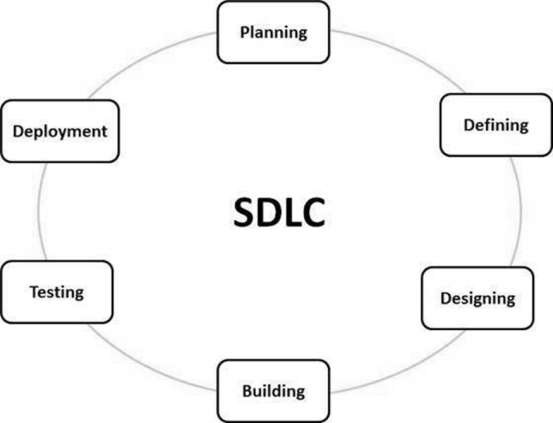
\includegraphics[scale=0.65]{Images/sdlc_stages.jpg}
    \caption{Software Development Life Cycle Overview}
    \label{fig:sdlc_cycle}
\end{figure}

\subsubsection*{Key Development Challenges}
Modern software development faces several critical challenges:

\begin{itemize}
    \item \textbf{Scalability Issues:} Maintaining consistent coding standards and best practices becomes increasingly difficult as teams grow, particularly without automated assistance.
    
    \item \textbf{Quality Assurance Gaps:} Traditional QA relies heavily on human review, introducing delays and inconsistent feedback timing.
    
    \item \textbf{Technical Debt Accumulation:} Without timely guidance, developers may adopt patterns that violate best practices, leading to accumulating technical debt.
    
    \item \textbf{Knowledge Transfer Challenges:} New team members often learn framework-specific conventions and best practices through trial and error, slowing onboarding and introducing variability.
\end{itemize}

\subsubsection*{Modern Development Approaches}
Contemporary practices aim to mitigate these challenges:

\begin{itemize}
    \item \textbf{Agile Methodologies:} Emphasize iterative development, continuous feedback, and rapid adaptation to changing requirements.
    
    \item \textbf{DevOps Integration:} Combines development and operations practices to enable continuous integration, automated testing, and real-time monitoring.
    
    \item \textbf{AI-Enhanced Development:} Emerging AI technologies provide intelligent assistance throughout the development process, from code generation to quality assurance.
\end{itemize}

These approaches lay the foundation for understanding how AI can address persistent challenges in code quality and consistency across modern software teams.

\subsection{Artificial Intelligence in Software Development}

\subsubsection*{Foundational AI Concepts}
Artificial Intelligence (AI) refers to computational systems capable of performing tasks that typically require human intelligence, such as reasoning, learning, problem-solving, and decision-making. AI encompasses a broad spectrum of techniques and paradigms with distinct capabilities and applications. Figure~\ref{fig:ai_hierarchy} provides a visual hierarchy of AI technologies.

\begin{figure}[H]
    \centering
    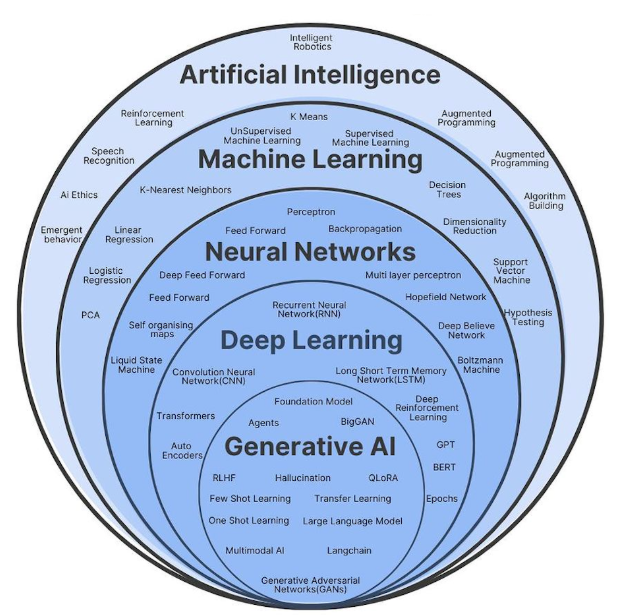
\includegraphics[scale=0.6]{Images/AI.png}
    \caption{Hierarchy of AI Technologies}
    \label{fig:ai_hierarchy}
\end{figure}

Key categories include:

\begin{itemize}
    \item \textbf{Symbolic AI:} Rule-based systems for reasoning and knowledge representation.
    \item \textbf{Machine Learning (ML):} Algorithms that learn from data to improve task performance.
    \item \textbf{Deep Learning (DL):} Neural networks with multiple layers capable of modeling complex patterns.
    \item \textbf{Generative AI:} Systems that produce new content, such as text or code, by learning patterns from existing datasets.
\end{itemize}

\subsubsection*{The AI Revolution in Software Engineering}
As software development becomes increasingly complex, traditional approaches struggle to maintain quality while meeting delivery deadlines. AI technologies offer transformative opportunities by embedding intelligent assistance directly into the development workflow.

Industry adoption illustrates this impact: surveys indicate that AI-generated code accounts for a significant portion of development output in major tech organizations~\cite{google2024ai_code, google2024developer_survey}. AI integration addresses critical business challenges, including maintaining code quality, reducing technical debt, and scaling development practices across growing teams. This shift defines the AI-Enhanced SDLC, a lifecycle where intelligent assistance is embedded throughout all phases.

\subsubsection*{Large Language Models (LLMs)}
LLMs represent a breakthrough in generative AI, trained on extensive natural language and code corpora. Unlike traditional tools, they understand context, semantics, and intent, enabling complex reasoning across domains. Figure~\ref{fig:llm_overview} shows a chronological overview of LLM development from 2018–2024.

\begin{figure}[H]
    \centering
    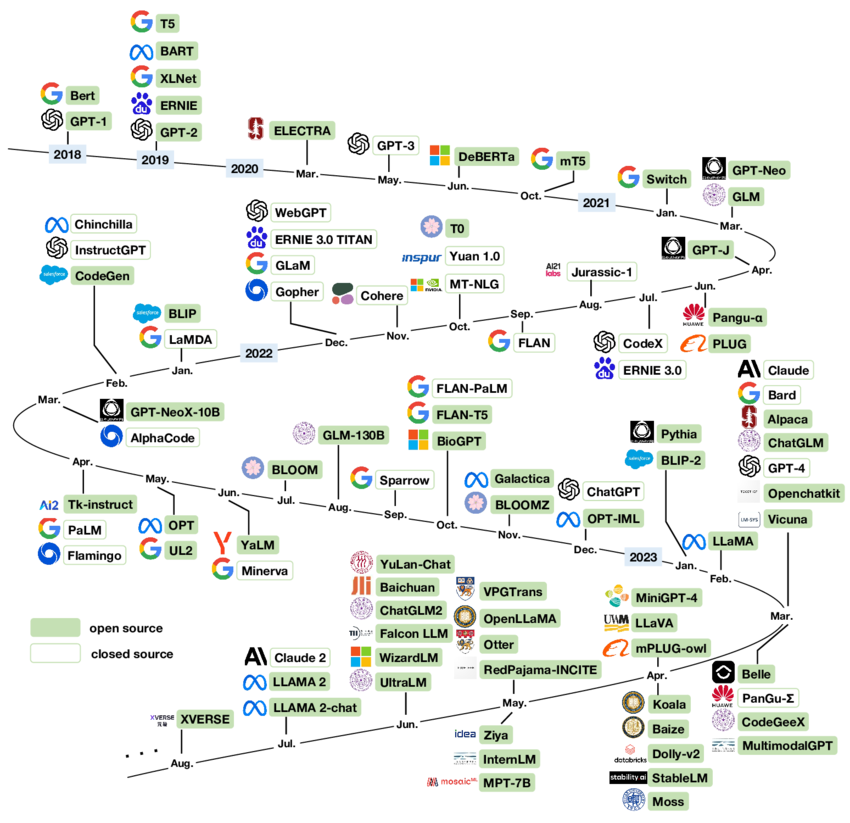
\includegraphics[scale=1]{Images/A-chronological-overview-of-large-language-models-LLMs-multimodal-and-scientific.png}
    \caption{Chronological Overview of Large Language Models (LLMs)}
    \label{fig:llm_overview}
\end{figure}

LLM capabilities include:

\begin{itemize}
    \item \textbf{Natural Language Understanding}
    \item \textbf{Pattern Recognition}
    \item \textbf{Content Generation}
    \item \textbf{Reasoning and Inference}
\end{itemize}

Applied to software development, these translate into:

\begin{itemize}
    \item \textbf{Contextual Code Analysis}
    \item \textbf{Intelligent Code Generation}
    \item \textbf{Explanatory Documentation}
    \item \textbf{Semantic Standards Enforcement}
\end{itemize}

\subsubsection*{AI Agents}
AI agents build on LLMs by autonomously reasoning, planning, and executing development tasks. They orchestrate LLM capabilities within workflows, providing seamless integration into IDEs, testing frameworks, and version control systems. Figure~\ref{fig:ai_agent_workflow} illustrates the agent architecture and orchestration workflow.

\begin{figure}[H]
    \centering
    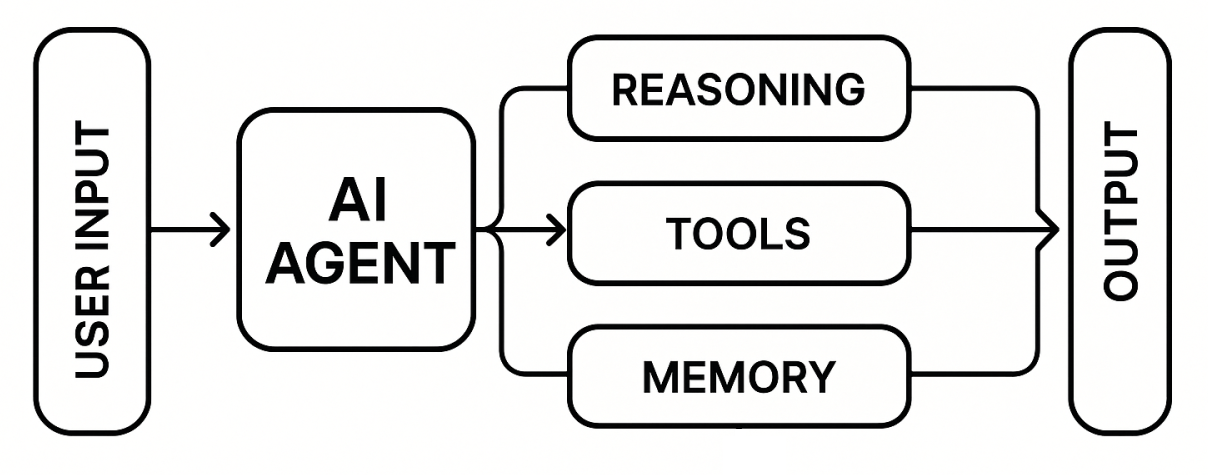
\includegraphics[scale=0.2]{Images/ai_agent.png}
    \caption{AI Agent Architecture and Orchestration Workflow}
    \label{fig:ai_agent_workflow}
\end{figure}

Core components include:

\begin{itemize}
    \item Code Analysis Engine
    \item Contextual Reasoning
    \item Development Tool Integration
    \item Contextual Adaptation via system prompts
    \item Feedback and Explanation System
\end{itemize}

\subsubsection*{Balancing AI Capabilities and Practical Considerations}
\textbf{Capabilities:}
\begin{itemize}
    \item Contextual Understanding
    \item Automated Analysis
    \item Intelligent Recommendations
    \item Project-specific Adaptation
\end{itemize}

\textbf{Limitations:}
\begin{itemize}
    \item Computational Cost
    \item Context Constraints
    \item Accuracy Considerations
    \item Integration Complexity
    \item Adaptation via prompts rather than continuous learning
\end{itemize}

\subsubsection*{AI-Enhanced SDLC}
The combination of LLMs and AI agents enables proactive, intelligent assistance throughout the entire software development lifecycle. This AI-enhanced SDLC transforms traditional development practices by embedding guidance, analysis, and automated support at each phase.

\paragraph{Transformative Impact on Development Practices}
\begin{itemize}
    \item \textbf{From Reactive to Proactive:} Traditional workflows provide feedback mainly during code reviews or testing phases. AI-enhanced systems deliver guidance during coding, design, and planning, preventing issues before they become embedded in the codebase and reducing the need for extensive refactoring.
    
    \item \textbf{From Inconsistent to Scalable:} Human-based quality assurance can vary in expertise and availability. AI agents provide consistent, expert-level analysis across large teams and codebases, ensuring uniform adherence to best practices and internal framework conventions.
    
    \item \textbf{From Static to Adaptive:} Unlike rule-based tools, AI adapts to project-specific patterns, team preferences, and evolving best practices, offering context-aware suggestions tailored to the particular codebase.
    
    \item \textbf{From Isolated to Integrated:} Instead of treating quality assurance and guidance as separate phases, AI agents integrate intelligent support directly into developer workflows, bridging planning, implementation, testing, and maintenance.
\end{itemize}

\paragraph{AI Applications Across the SDLC}
AI technologies provide targeted assistance at each SDLC phase, addressing specific challenges and improving efficiency:

\begin{itemize}
    \item \textbf{Requirements and Planning:} AI analyzes historical project data to estimate timelines, identify ambiguities in requirements, and suggest optimal resource allocation. Natural language processing helps translate business requirements into technical specifications with higher precision.
    
    \item \textbf{Design and Architecture:} AI assists architects by analyzing existing codebases, recommending architectural patterns, detecting design anti-patterns, and ensuring alignment with organizational standards. This reduces the likelihood of systemic flaws early in the project lifecycle.
    
    \item \textbf{Implementation:} During coding, AI agents provide context-aware code completions, enforce framework-specific best practices, detect potential bugs, and suggest refactoring opportunities. This reduces rework, accelerates development, and supports consistent code quality.
    
    \item \textbf{Testing and Quality Assurance:} AI generates comprehensive test cases, identifies edge cases that might be missed manually, prioritizes test execution based on risk, and evaluates code quality against defined standards. This enhances reliability and reduces technical debt accumulation.
    
    \item \textbf{Deployment and Maintenance:} AI monitors deployment health, predicts potential issues, and recommends optimizations based on performance metrics and usage patterns. Continuous insights help maintain system stability and inform future development iterations.
\end{itemize}

Overall, the AI-enhanced SDLC shifts the development workflow from reactive and fragmented practices toward a more proactive, adaptive, and integrated approach. By embedding intelligent assistance at every stage, it directly addresses the challenges of scaling teams, maintaining consistent quality, and supporting internal framework-specific best practices—core objectives of this project.

\section{State of the Art and Existing Solutions}

This section examines both market-available solutions (state of the art) and environment-specific approaches (existing solutions) to understand the current landscape of code quality and best practices enforcement.

\subsection{State of the Art: Market Solutions}

The software development market offers various AI-powered tools and platforms that aim to enhance code quality and developer productivity. These solutions represent the current state of the art in intelligent development assistance:

\paragraph{AI-Powered Code Analysis Tools}
Commercial and open-source solutions provide intelligent code analysis capabilities:

\begin{itemize}
    \item \textbf{AI Code Assistants:} Tools like GitHub Copilot, Amazon CodeWhisperer, and Tabnine provide AI-powered code completion and generation, helping developers write code more efficiently.
    
    \item \textbf{AI-Powered IDEs:} Modern development environments like Cursor and Claude Code integrate AI assistance directly into the coding workflow, offering context-aware code generation, refactoring, and intelligent suggestions.
    
    \item \textbf{Static Analysis Platforms:} Solutions such as SonarQube, CodeClimate, and DeepCode offer automated code quality analysis with AI-enhanced pattern detection.
    
    \item \textbf{AI Code Review Tools:} Platforms like PullRequest.com and CodeRabbit provide AI-assisted code review capabilities, offering automated suggestions and quality assessments.
\end{itemize}

\paragraph{Market Solution Capabilities}
These market solutions typically offer:

\begin{itemize}
    \item \textbf{General Code Analysis:} Broad pattern recognition and quality assessment across multiple programming languages and frameworks.
    
    \item \textbf{AI-Powered Suggestions:} Intelligent recommendations for code improvements, refactoring, and best practices.
    
    \item \textbf{Integration with Popular IDEs:} Seamless integration with widely-used development environments like VS Code, IntelliJ, and Eclipse.
\end{itemize}

\subsection{Existing Solutions: Environment-Specific Approaches}

Within our specific development environment, software engineers currently rely on a combination of modern AI-powered tools and traditional approaches to maintain code quality and enforce best practices:

\paragraph{Current Feedback Mechanisms}
The existing approaches in our environment can be categorized into several key mechanisms:

\begin{itemize}    
    
    \item \textbf{Code Reviews:} Human reviewers examine code for design quality, readability, maintainability, and adherence to standards. While this approach provides high-level, context-aware feedback, it often introduces delays and requires significant effort.
    
    \item \textbf{Presubmit Checks:} Automated scripts that validate code before submission, enforcing style guides, ensuring compilation, and verifying simple correctness and safety constraints. Although fast and reliable, they primarily focus on surface-level checks and do not consider design or contextual issues.
    
    \item \textbf{Coding Assistant:} Our internal IDE includes an integrated coding assistant that provides AI-powered code completion, generation, and basic suggestions to help developers write code more efficiently.

    \item \textbf{Linters:} Live IDE-integrated linters that catch style issues, deprecations, and basic code quality problems in real-time as developers write code. These tools provide immediate feedback on syntax, formatting, and some best practices.

    \item \textbf{Rule-Based Checks:} Systems that enforce coding conventions, naming schemes, and formatting standards. These tools provide consistency and objectivity but cannot reason about complex or context-dependent best practices.
\end{itemize}

\paragraph{Gap Analysis: Market vs. Environment Solutions}

While both market solutions and environment-specific approaches provide valuable capabilities, they leave significant gaps in addressing internal framework-specific best practices:

\textbf{Market Solution Limitations:}
\begin{itemize}
    \item \textbf{Generic Analysis:} Market tools provide general code quality analysis but lack deep understanding of internal framework-specific conventions and patterns.
    
    \item \textbf{External Dependency:} Commercial solutions require external data sharing and may not align with internal security and privacy requirements.
    
    \item \textbf{Limited Customization:} Generic tools cannot be easily customized to enforce internal-specific best practices and architectural patterns.
\end{itemize}

\textbf{Environment Solution Limitations:}
While our environment includes a coding assistant and live linters, there remains a significant gap in providing intelligent feedback specifically for internal framework best practices during the active coding phase. This timeline illustrates where current feedback mechanisms fit into the developer workflow:

\begin{figure}[H]
    \centering
    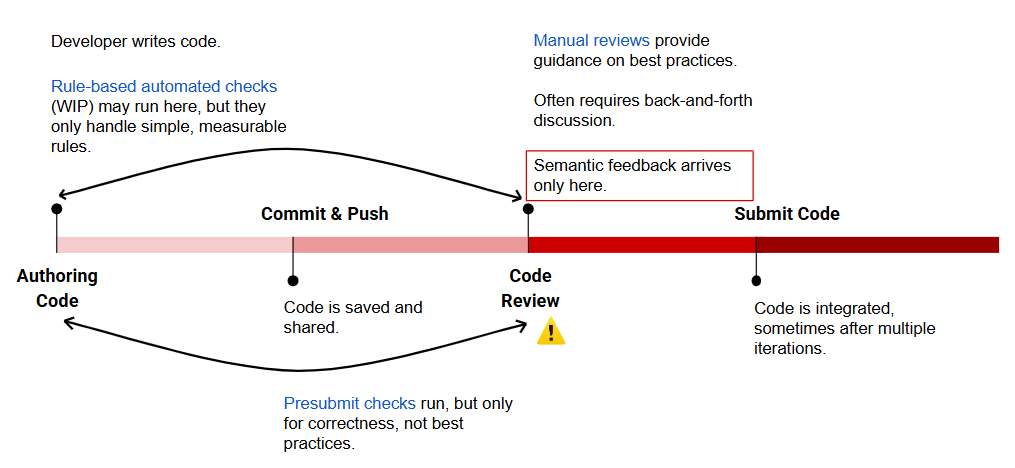
\includegraphics[scale=0.9]{Images/developer_workflow_feedback_timeline.png}
    \caption{Current Developer Workflow Feedback Timeline}
    \label{fig:developer_workflow_feedback_timeline}
\end{figure}

During the \textbf{Coding Phase}, developers get support from the Coding Assistant for code generation and completion, and from Linters for style issues and deprecations. However, these tools focus on general coding assistance and basic quality checks rather than internal framework-specific best practices.

The most insightful feedback on design and best practices typically comes during \textbf{Code Review}, but this happens after the initial development, making changes more disruptive.

Finally, \textbf{Presubmit Checks} before submission focus on correctness and safety, not on proactive best practice guidance.

This leaves a significant gap: there's no real-time, intelligent support for adhering to internal framework best practices while the developer is actively coding, which is the gap our project aims to fill.

\begin{table}[H]
\centering
\begin{tabular}{|p{4cm}|p{5cm}|p{5cm}|}
\hline
\textbf{Approach} & \textbf{Strengths} & \textbf{Limitations} \\
\hline
Code Reviews & Context-aware, high-level insights & Feedback delayed, time-consuming \\
\hline
Presubmit Checks & Fast, automated validation & Limited scope, mostly syntax and safety \\
\hline
Coding Assistant & AI-powered code generation, completion & General assistance, not framework-specific \\
\hline
Linters & Real-time style and deprecation checks & Basic quality only, not best practices \\
\hline
Rule-Based Checks & Consistency, objectivity & Cannot handle complex or contextual practices \\
\hline
\end{tabular}
    \caption{Comparison of available software quality support solutions}
\label{tab:extended_solutions}
\end{table}

    
\paragraph{Impact of Delayed Feedback}
Following from the previous analysis, these workflow issues create concrete impacts on development:

\begin{itemize}
    \item \textbf{Technical Debt Accumulation:} Delayed feedback and limited enforcement of best practices lead to accumulating technical debt and inconsistencies in code quality over time.
    
    \item \textbf{Prolonged Review Cycles:} Review cycles take longer because developers must iterate multiple times to address issues discovered late in the process.
    
    \item \textbf{Developer Frustration:} The repetitive cycle of late-stage corrections contributes to developer frustration and reduced productivity.
    
    \item \textbf{Inconsistent Quality Standards:} Without real-time guidance, adherence to best practices varies significantly across team members and projects.
    
    \item \textbf{Increased Development Costs:} The cost of fixing issues increases exponentially the later they are discovered in the development process.
\end{itemize}

This analysis clearly demonstrates why we need a solution that brings intelligent best practices guidance earlier, directly into the authoring process, addressing the specific gap in internal framework best practices enforcement that current approaches cannot fill.




\paragraph{Opportunity for Framework-Specific AI Solutions}

The analysis reveals a clear opportunity for developing framework-specific AI solutions that combine the intelligence of market tools with the specificity required for YouTube framework best practices. While market solutions provide general AI capabilities and environment solutions offer domain knowledge, neither adequately addresses the need for real-time, intelligent feedback tailored to YouTube framework conventions.

This gap creates a compelling case for integrating LLM-powered assistance directly into the YouTube development workflow, providing intelligent, context-aware guidance that understands both general best practices and YouTube-specific patterns.

---

\section{Project Requirements}

To tackle the issue of delayed feedback and limited intelligent assistance, our solution integrates the power of large language models directly into the developer's workflow in the IDE.

The proposed system builds on gaps identified in existing solutions. It aims to provide real-time, AI-driven feedback directly in the developer workflow, while maintaining performance, scalability, and usability.

\subsection{Functional Requirements}
The system must:
\begin{itemize}
    \item \textbf{Detect Framework Violations:} Identify violations of internal YouTube framework best practices and coding standards in real-time during development.
    
    \item \textbf{Provide Contextual Explanations:} Explain violations in clear, developer-friendly language with context-specific rationale that helps developers understand why certain patterns are problematic.
    
    \item \textbf{Generate Actionable Fixes:} Suggest specific, actionable fixes leveraging AI-generated solutions tailored to YouTube framework patterns and conventions.
    
    \item \textbf{Enable Developer Interaction:} Allow developers to accept, reject, or modify AI suggestions, providing full control over the implementation of recommended changes.
    
    \item \textbf{Maintain Contextual Relevance:} Ensure feedback appears in the appropriate location within the code and remains relevant and accurate as the developer continues coding.
    
    \item \textbf{Seamless IDE Integration:} Integrate seamlessly with the existing internal IDE, extension, and backend workflow without disrupting the developer's current development process.
\end{itemize}

\subsection{Non-Functional Requirements}
The system should also meet broader quality criteria:
\begin{itemize}
    \item \textbf{Performance:} Provide fast, near real-time responses to avoid interrupting developer workflow.
    \item \textbf{Scalability:} Efficiently handle large codebases and multiple simultaneous users.
    \item \textbf{Maintainability:} Enable modular updates, addition of new AI models, or coding rules.
    \item \textbf{Reliability:} Ensure robustness in production environments with minimal downtime.
    \item \textbf{Security and Privacy:} Comply with organizational policies, ensuring safe handling of code and data.
    \item \textbf{Usability:} Deliver concise, context-aware, and minimally intrusive feedback.
    \item \textbf{Extensibility:} Easily add new rules, models, or integrations.
\end{itemize}

\begin{table}[H]
\centering
\begin{tabular}{|p{6cm}|p{8cm}|}
\hline
\textbf{Requirement Type} & \textbf{Description} \\
\hline
Functional & Framework violation detection, contextual explanations, actionable fixes, developer interaction, contextual relevance, seamless IDE integration \\
\hline
Non-Functional & Performance, scalability, maintainability, reliability, security, usability, extensibility \\
\hline
\end{tabular}
\caption{Summary of project requirements}
\label{tab:extended_requirements}
\end{table}

\paragraph{Rationale}
These requirements address limitations identified in existing solutions by embedding proactive, context-aware feedback directly in the coding workflow, specifically targeting YouTube framework best practices. This approach enhances developer productivity, reduces framework-specific errors, and supports consistent adherence to internal YouTube development standards.


\section*{Conclusion}
This chapter established the business and theoretical foundation for integrating AI into YouTube framework development workflows. Beginning with an analysis of modern development challenges, it identified key issues in maintaining code quality and consistency across growing teams. The exploration of AI technologies—particularly Large Language Models and AI agents—revealed their potential for addressing these challenges through proactive, context-aware assistance.

The examination of both market solutions and environment-specific approaches highlighted significant limitations: market tools lack framework-specific knowledge, while traditional environment solutions provide delayed feedback and limited scope. There remains a critical gap in delivering real-time, intelligent assistance tailored to YouTube framework best practices.

The project requirements defined in this chapter focus on bridging this gap through real-time, AI-driven feedback that integrates seamlessly into the YouTube development workflow. The proposed solution combines the intelligence of modern AI technologies with the specificity required for YouTube framework conventions, setting the stage for the detailed system design presented in the following chapter.  








%==============================================================================
\end{spacing}


